\chapter{Quá trình hiện thực}
Từ giới hạn đề tài và cơ sở lý thuyết, ta chia quá trình hiện thực thành ba phần tương đối độc lập:
\begin{itemize}
    \item Hiện thực quá trình xác định vùng biển số và vùng ký tự.
    \item Hiện thực BNN nhận dạng các ký tự đã tìm được.
    \item Tạo overlay gia tốc cho quá trình xác định vùng biển số và vùng ký tự.
\end{itemize}

\section{LP Detection and Character Segmentation}
\section{Character Regcongition}
\section{Tạo overlay gia tốc cho quá trình xác định vùng biển số và ký tự}
Từ quá trình hiện thực tim vùng biển số và ký tự ta có thể thấy, hàm gắn nhãn đối tượng được sử dụng thường xuyên. Vì vậy, để khai thác tính tái sử dụng cho overlay, nhóm quyết định chọn hàm gắn nhãn đối tượng cho việc tạo overlay.

    \subsection{Hàm gắn nhãn đối tượng}
    \textbf{Về hàm cần gia tốc: skimage.measure.label}
    
    Hàm skimage.measure.label(input[, neighbors, …]) là hàm ngắn nhãn những vùng được liên kết với nhau trong một mảng số nguyên (ví dụ: ảnh nhị phân).
    
    Chi tiết về hàm xem tại: \url{https://scikit-image.org/docs/dev/api/skimage.measure.html#skimage.measure.label}
    
    \textbf{Chức năng hàm gia tốc hw\_label\_accel}
    
    Protype của hàm:
    hw\_label\_accel(axis\_t *src, axis\_t *dst, int rows, int cols).
    
    Trong đồ án này, đầu vào của hàm là một ảnh nhị phân (ma trận 2 chiều) nên chức năng của hàm trở nên đơn giản hơn so với hàm skimage.measure.label() về:
    \begin{itemize}
        \item input: input của hw\_label\_accel (src) là ảnh nhị phân hay một mảng các giá trị nguyên trong khi input của skimage.measure.label() có thể là ma trận 2 hay 3 chiều.
        \item neighbors: Một điểm trong input của hw\_label\_accel có số hàng xóm tối đa luôn là 8 thay vì có thể là 4 hoặc 8.
        \item background: Nền trong input của hw\_label\_accel luôn có giá trị là 0 thay vì có thể lựa chọn.
        \item Returns: Giá trị trả về của hw\_label\_accel (dst)là một mảng số nguyên hay một ảnh xám. Nó đồng nhất với giá trị trả về của skimage.measure.label (labels).
    \end{itemize}
    
    \subsection{Giải thuật của hàm gia tốc}
    
    Hình \ref{fig:overlayalgorithmflow} thể hiện giải thuật cho hàm hw\_label\_accel. Trong đó:
    \begin{itemize}
        \item Hàm ismarked(src[i]) trả về TRUE nếu điểm i đã được gắn nhãn và FALSE nếu chưa.
        \item Hàm mark(src[idx]) sẽ gắn nhãn cho giá trị tại điểm idx. Giá trị của nhãn phụ thuộc vào số lượng nhãn đã được sử dụng.
        \item Hàm FB\_neighbors(i) trả về những điểm kế của i mà tại đó src[i] chưa được gắn nhãn.
    \end{itemize}
    Kết thúc hàm ta sẽ thu đươc src là output cần tìn. Ta cần đầy src ra ngõ ra.
    \begin{figure}[htp]
    	\centering
     	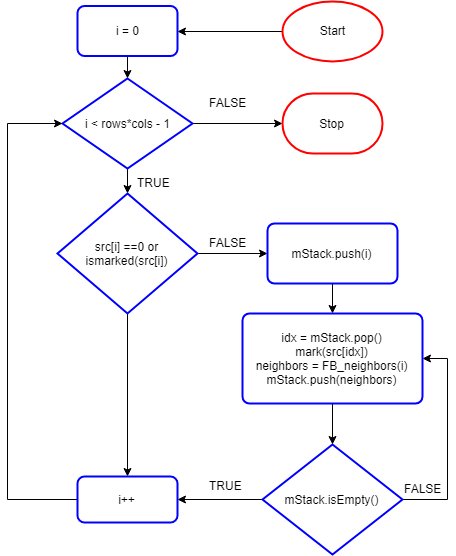
\includegraphics[scale=.8]{images/overlay_algo_flow.png}
    	\caption{Giải thuật cho hàm hw\_label\_accel}
    	\label{fig:overlayalgorithmflow}
    \end{figure}
    
    \subsection{Hiện thực hàm hw\_label\_accel bằng Vivado HLS}
    